\section{Theorie}	
%
\subsection{Gleichstrom - Wechselstrom - Effektivwert}
%
Im Gegensatz zum Gleichstrom fließt bei dem Wechselstrom der Strom nicht konstant in eine Richtung, sondern verläuft (meist) sinusförmig. Dementsprechend ist auch die Potentialdifferenz nicht in ihrem Vorzeichen konstant. Dies bedeutet, dass die Spannung ständig umgepohlt wird und somit der Strom der Spannung mit der Phasenverschiebung $\varphi$ zeitlich versetzt folgt.
%
\begin{figure}[H]
	\begin{center}
		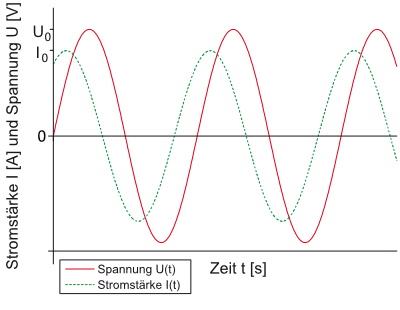
\includegraphics[width=18em]{wechselstrom}
	\end{center}
	\caption{Symbolischer, zeitlicher Verlauf von Wechselspannung und Wechselstrom}
\end{figure}
%
Die dargestellten Kurven lassen sich mithilfe der Formeln
%
\begin{align}
	U(t) &= U_0 \sin \omega t\\
	I(t) &= I_0 \sin(\omega t + \varphi)
\end{align}
%
beschreiben.\\
Der \textit{Effektivwert} beschreibt einen quadratischen Mittelwert einer zeitlich veränderlichen physikalischen Größe. Im Falle des Wechselstroms beschreibt er den Wert des Gleichstroms, welcher an einem ohmschen Widerstand die gleiche Leistung erziehlen würde. Somit lässt sich der Effektivwert mathematisch als die Wurzel des quadrierten zeitlichen Mittelwertes der Größe beschreiben.
%
\begin{align}
	U_{eff} &= \sqrt{\overline{u^2(t)}}\\
	I_{eff} &= \sqrt{\overline{i^2(t)}}
\end{align}
%
($u(t)$ : zeitlicher Verlauf der Wechselspannung $U$, $i(t)$ : zeitlicher Verlauf des Wechselstroms $I$) (Demtröder, 2009, S.151)
%
\subsection{Impedanz und Phasenverschiebung}
%
Betrachtet man einen Stromkreis mit einer periodisch angelegten Wechselspannung $U$, einer Induktivität $L$, einer Kapazität $C$ und einem ohmschen Widerstand $R$, so gilt nach der Kirchhoffschen Regel folgende Beziehung (Nolting 3, S.234): 
%
\begin{align}
	U = L\dot{I}+RI+\frac{Q}{C} 
	\label{eq:1}
\end{align}
%
Ferner gilt der Zusammenhang zwischen Strom und Ladung
%
\begin{align}
	I = \dot{Q} = \frac{\text{d}Q}{\text{d}t}\text{,}
\end{align}
%
wodurch sich die Gleichung \ref{eq:1} zu einer Differenzialgleichung zweiter Ordnung von $I(t)$ umschreiben lässt.
%
\begin{align}
	L\ddot{I}+R\dot{I}+\frac{I}{C}= \dot{U}
\end{align}
%
Mittels der komplexen Lösungsansätze $U = U_0 e^{\text{i}\omega t}$ und $I = I_0 e^{\text{i}\omega t+\varphi}$ ergibt sich folgende Gleichung:
%
\begin{align}
	U\omega \text{i} = I(L\omega^2+R\omega \text{i}+\frac{1}{C})
\end{align}
%
Angepasst an die komplexe Schreibweise von $I$ und $U$, definiert man den komplexen Widerstand $Z=\frac{U}{I}$. Daraus folgt:
%
\begin{align}
	Z = \frac{U}{I} = R+\text{i}\left(\omega L - \frac{1}{\omega C}\right)
\end{align}
%
Diese Gleichung lässt sich als Vektor in der komplexen Ebene auffassen, wodurch die Impedanz der Betrag dieses Vektors ist und die Phasenverschiebung $\varphi$ durch die Gleichung 
%
\begin{align}
	\varphi = \arctan\left(\frac{\Im(Z)}{\Re(Z)}\right) = \arctan\left(\frac{\omega L - \frac{1}{\omega C}}{R}\right)
\end{align}
%
beschrieben werden kann.
